%!TEX root = SysSpec_ClockPendulumAnalyzer.tex
\subsection{Umsetzung Sensor} %TODO describe schemantic 1 and 2 each
	Die Aufbau der Messvorrichtung des Sensors und dessen Anschluss ist nach folgenden Kriterien erfolgt:
	\begin{itemize}
		\item Flexible Positionierung des Sensors in der Höhe.
		\item Kleine Baugrösse um auch in kleineren Uhren messen zu können.
		\item Möglichst einfacher Anschluss mit Sicherung gegen Fehler.
	\end{itemize}
	Für den Betrieb des in Kapitel \ref{cap:sensoren} beschriebenen IR-Sensors sind im Datenblatt die in Abbildung \ref{fig:info_SFH9201} Anschlüsse gegeben.
	\begin{figure}[H]
		\centering
		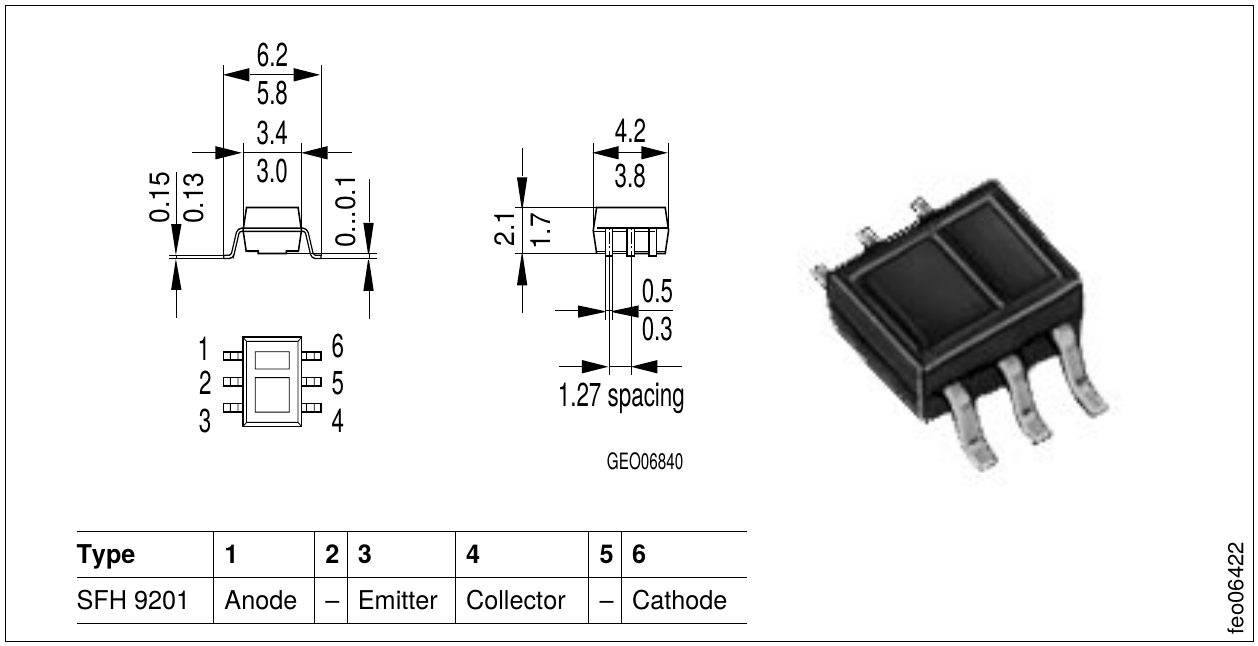
\includegraphics[width=.7\textwidth]{Sensor_layout}
		\caption{Anschlussinformationen SFH9201 (Bildquelle aus Datenblatt)}
		\label{fig:info_SFH9201}
	\end{figure}
	Weiter ist ein Schaltschema gegeben, welches den Grundaufbau der Schaltung vorgibt (Abbildung \ref{fig:schema_SFH9201}).
	\begin{figure}[H]
		\centering
		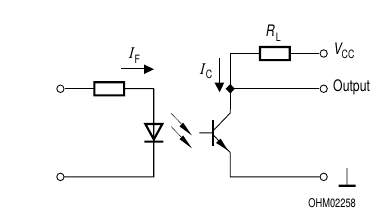
\includegraphics[width=.7\textwidth]{Sensor_Schema}
		\caption{Anschluss-Schema SFH9201 (Bildquelle aus Datenblatt)}
		\label{fig:schema_SFH9201}
	\end{figure}
	Da die Speisung der Diode und des Collectors in unserem Falle identisch sind, werden drei Anschlüsse benötigt. Eine Speisung mit 3.3V, ein Ausgang, um den Schaltzustand des Sensors zu ermitteln und ein Anschluss für Ground. Da es sich um einen analogen Sensor handelt, ist dem Ausgang des Sensors ein Schmitt-Trigger angehängt, welcher die Analoge Spannung in ein digitales Signal umwandelt. Da sich das Verhalten des Sensors, abhängig von der Reflektion des Pendels und des Abstandes zum Pendel, verändern kann, sind sowohl der Ausgangswiderstand für den Collector, wie auch der Vergleichswiderstand des Schmitt-Triggers, sowie der Widerstand der Hysterese des Schmitt-Triggers einstellbar gestaltet. Dies mittels Potentiometer. Um die Schaltung für jedes Pendel einfach, mittels visueller Hilfe, einstellen zu können, is eine grüne LED angebracht, die leuchtet, sobald das Pendel erkannt ist. Gemeinsam ist daher das in Abbildung \ref{fig:schema_sensor} dargestellte Schema entstanden.
	\begin{figure}[H]
		\centering
		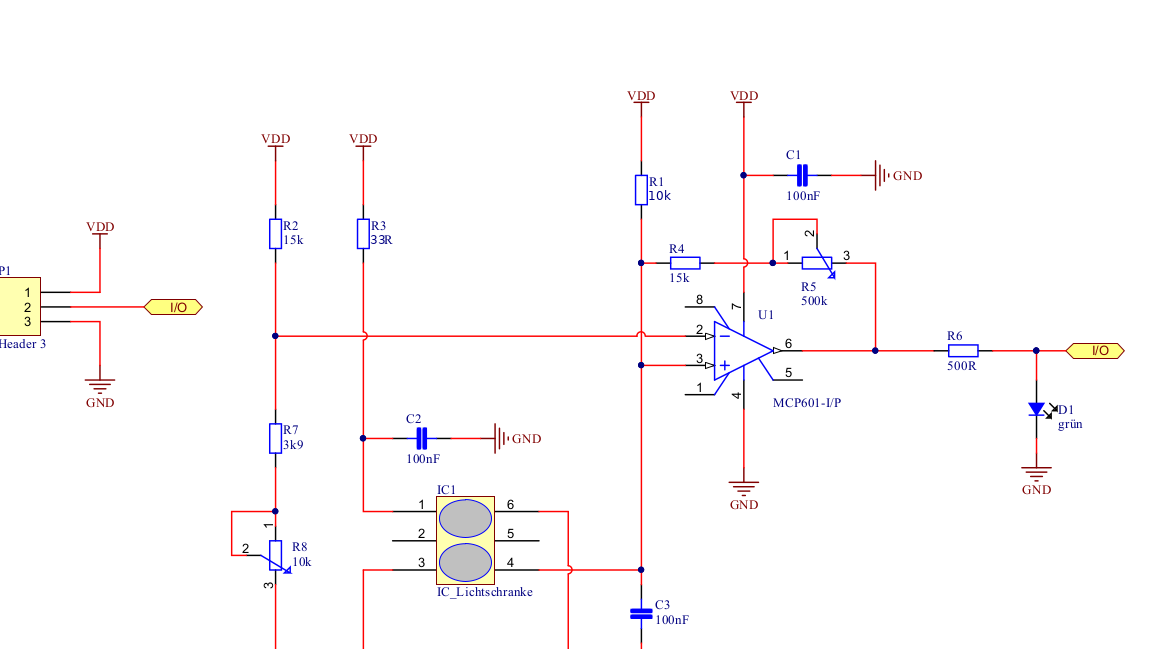
\includegraphics[width=.8\textwidth]{Circuit_Sensor}
		\caption{Ermitteltes Elektroschema für das Sensor-PCB SFH9201}
		\label{fig:schema_sensor}
	\end{figure}
	Die Diode vor dem Sensor verhindert ein falschs Anschliessen der IR-Diode und des Emitters. Der Widerstand von 24$\Omega$ ist der Vorgabe gemäss Datenblatt berechnet. Diese sind:
	\begin{itemize}
		\item 1.65V als maximale und gemessene Spannung $U_{IRD}$ über der IR-Diode
		\item 50mA Betriebsstrom $I_F$
	\end{itemize}
	Ausgehend von einer Speisung $U_S$ von 3.3V und einer Verlustspannung $U_V$ von 0.5V über der Sperrdiode ergibt dies folgende Formel:
	\[
		R = \frac{U_S - U_V - U_{IRD}}{I_R} = \frac{3.3 - 0.5 - 1.65}{0.05} = 23\Omega
	\]
	Die Werte für die Potentiometer wurden in Zusammenarbeit mit der Elektrotechnik ermittelt. Der 560$\Omega$ Widerstand dient als Schutz für den Sensor, falls das Potentiometer auf 0 gedreht wird. Ein entsprechendes PCB\footnote{Printed Circuit Board} ist an der Hochschule Luzern, Technik \& Archtektur erstellt worden.\\
	Als Stütze für den Sensor dient eine Holzkonstruktion, welche über ein Lochraster von 10mm verfügt, an welchen sich der Sensor befestigen lässt. So können verschiedene Pendellängen und Anordungen angedeckt werden (Abbildung \ref{fig:Sensor_overview}).
	\begin{figure}[H]
		\centering
		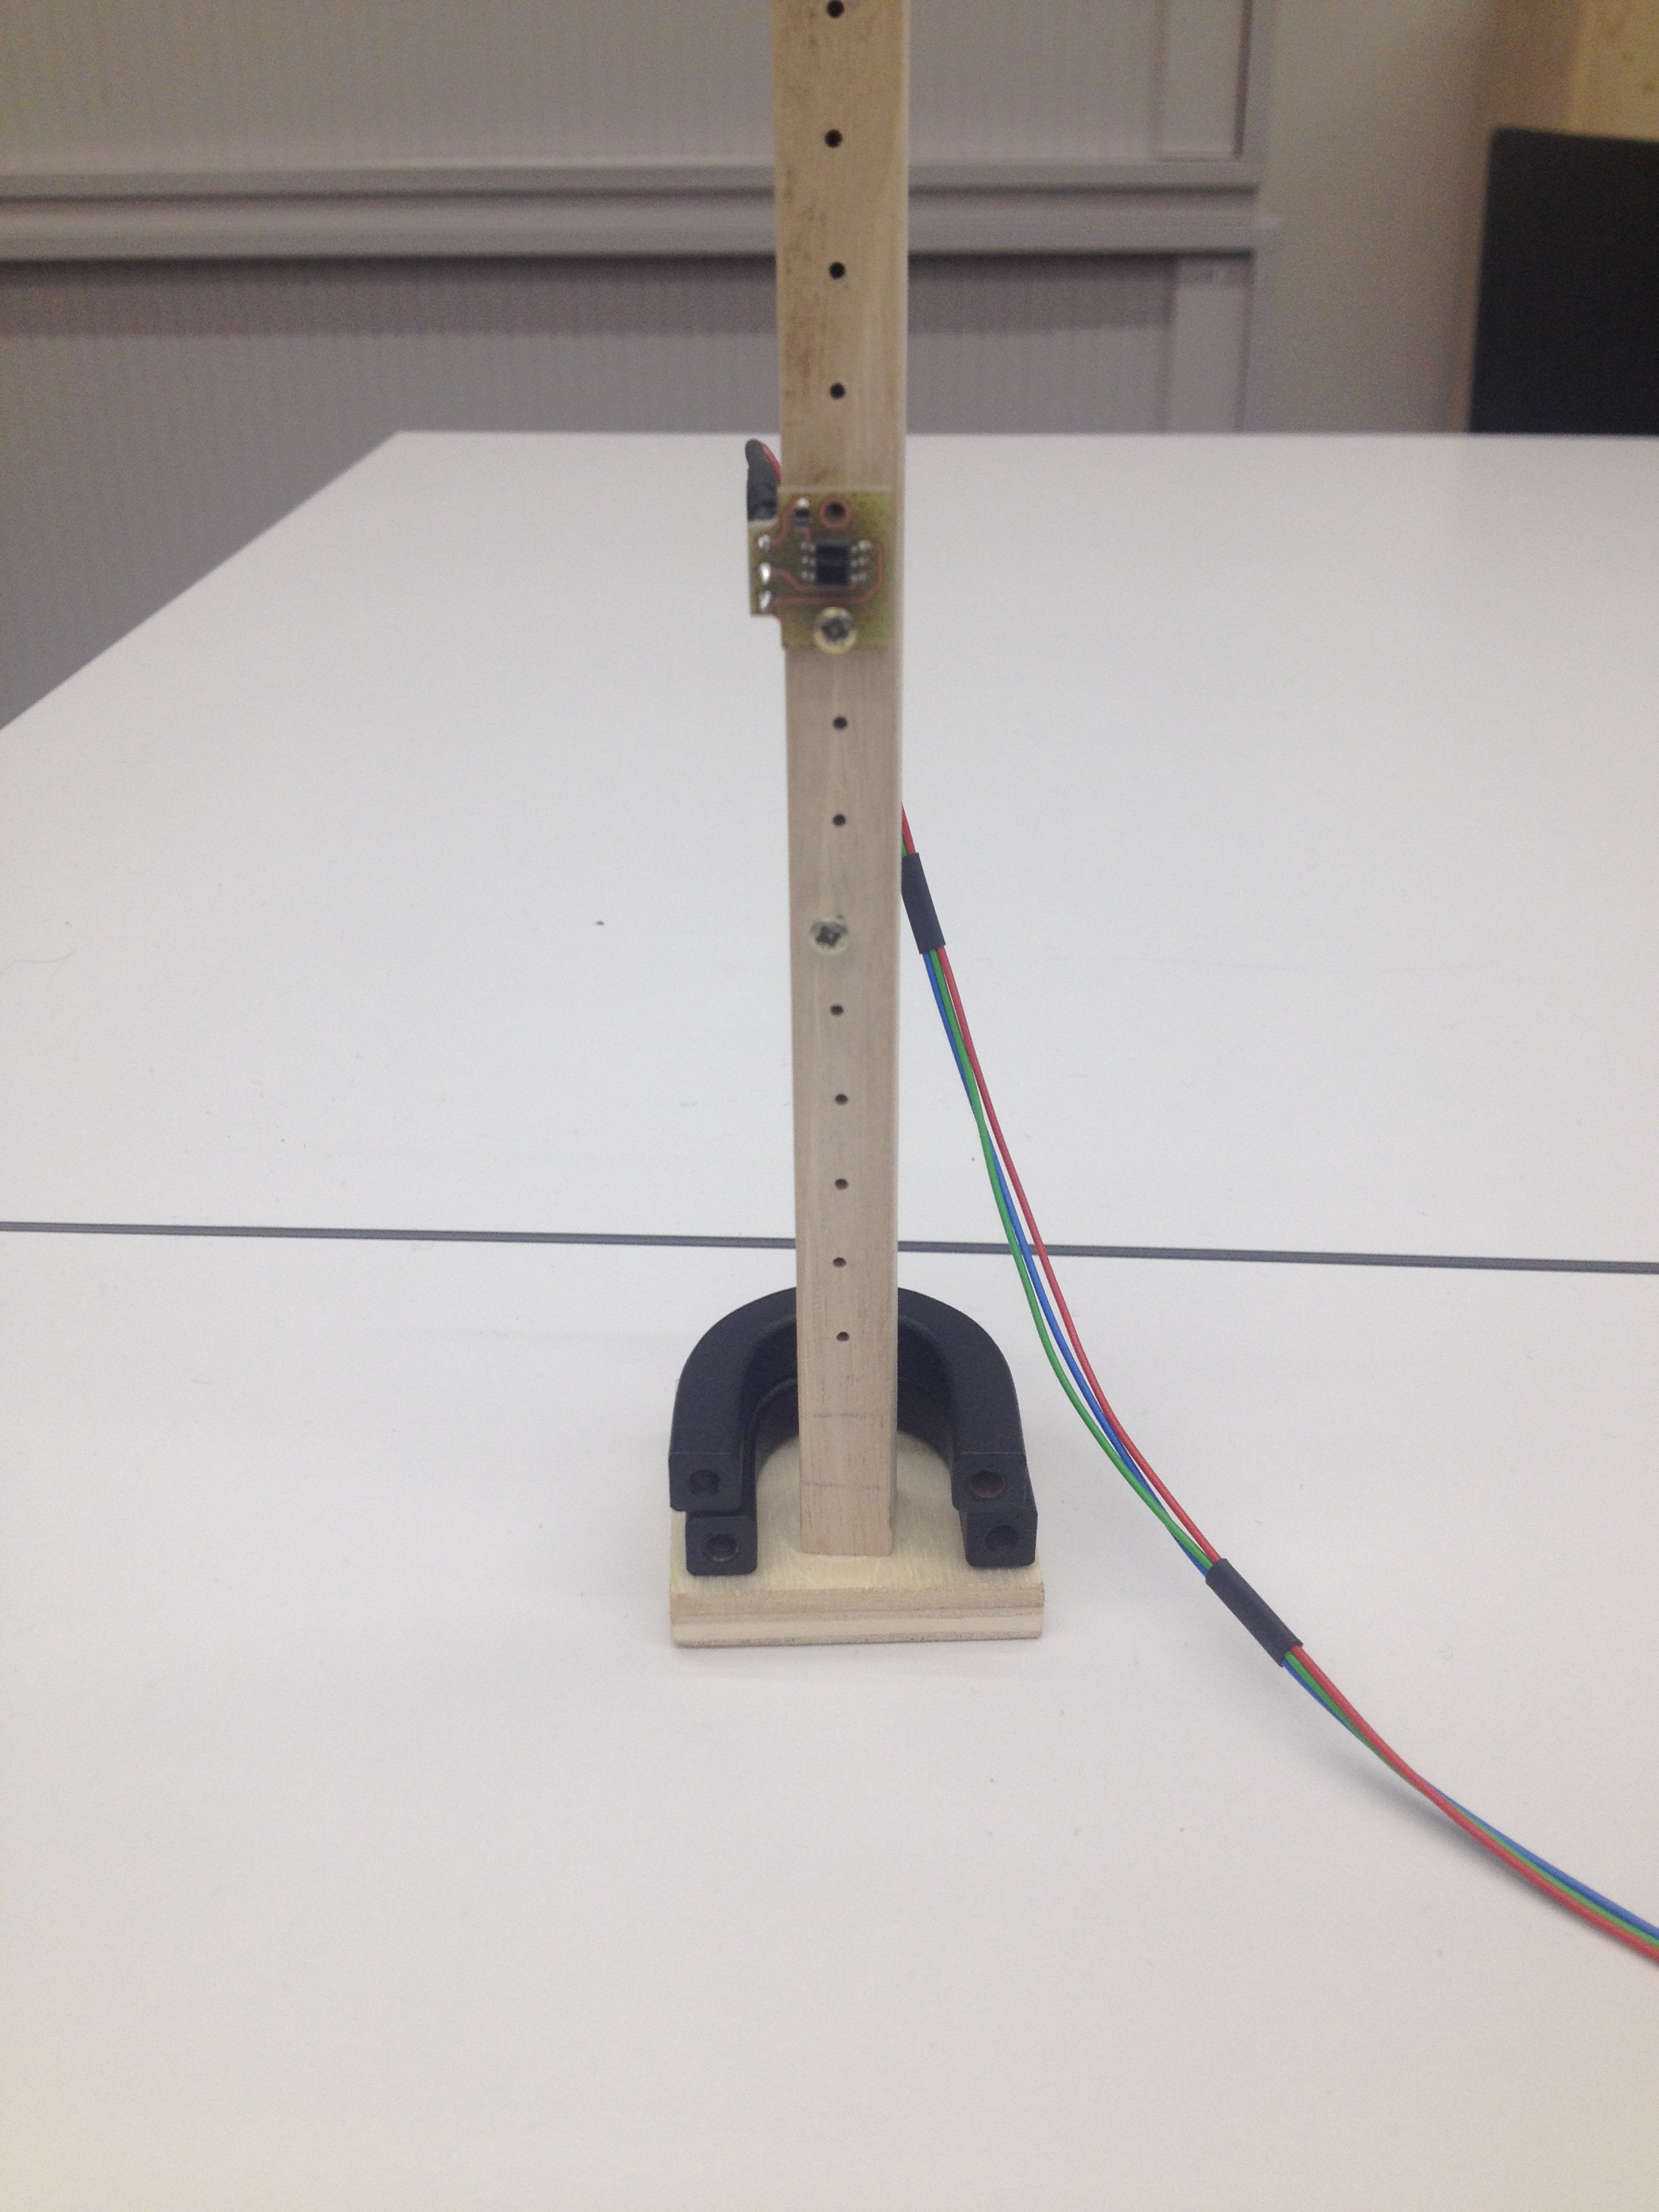
\includegraphics[width=.4\textwidth]{Sensor_overview}
		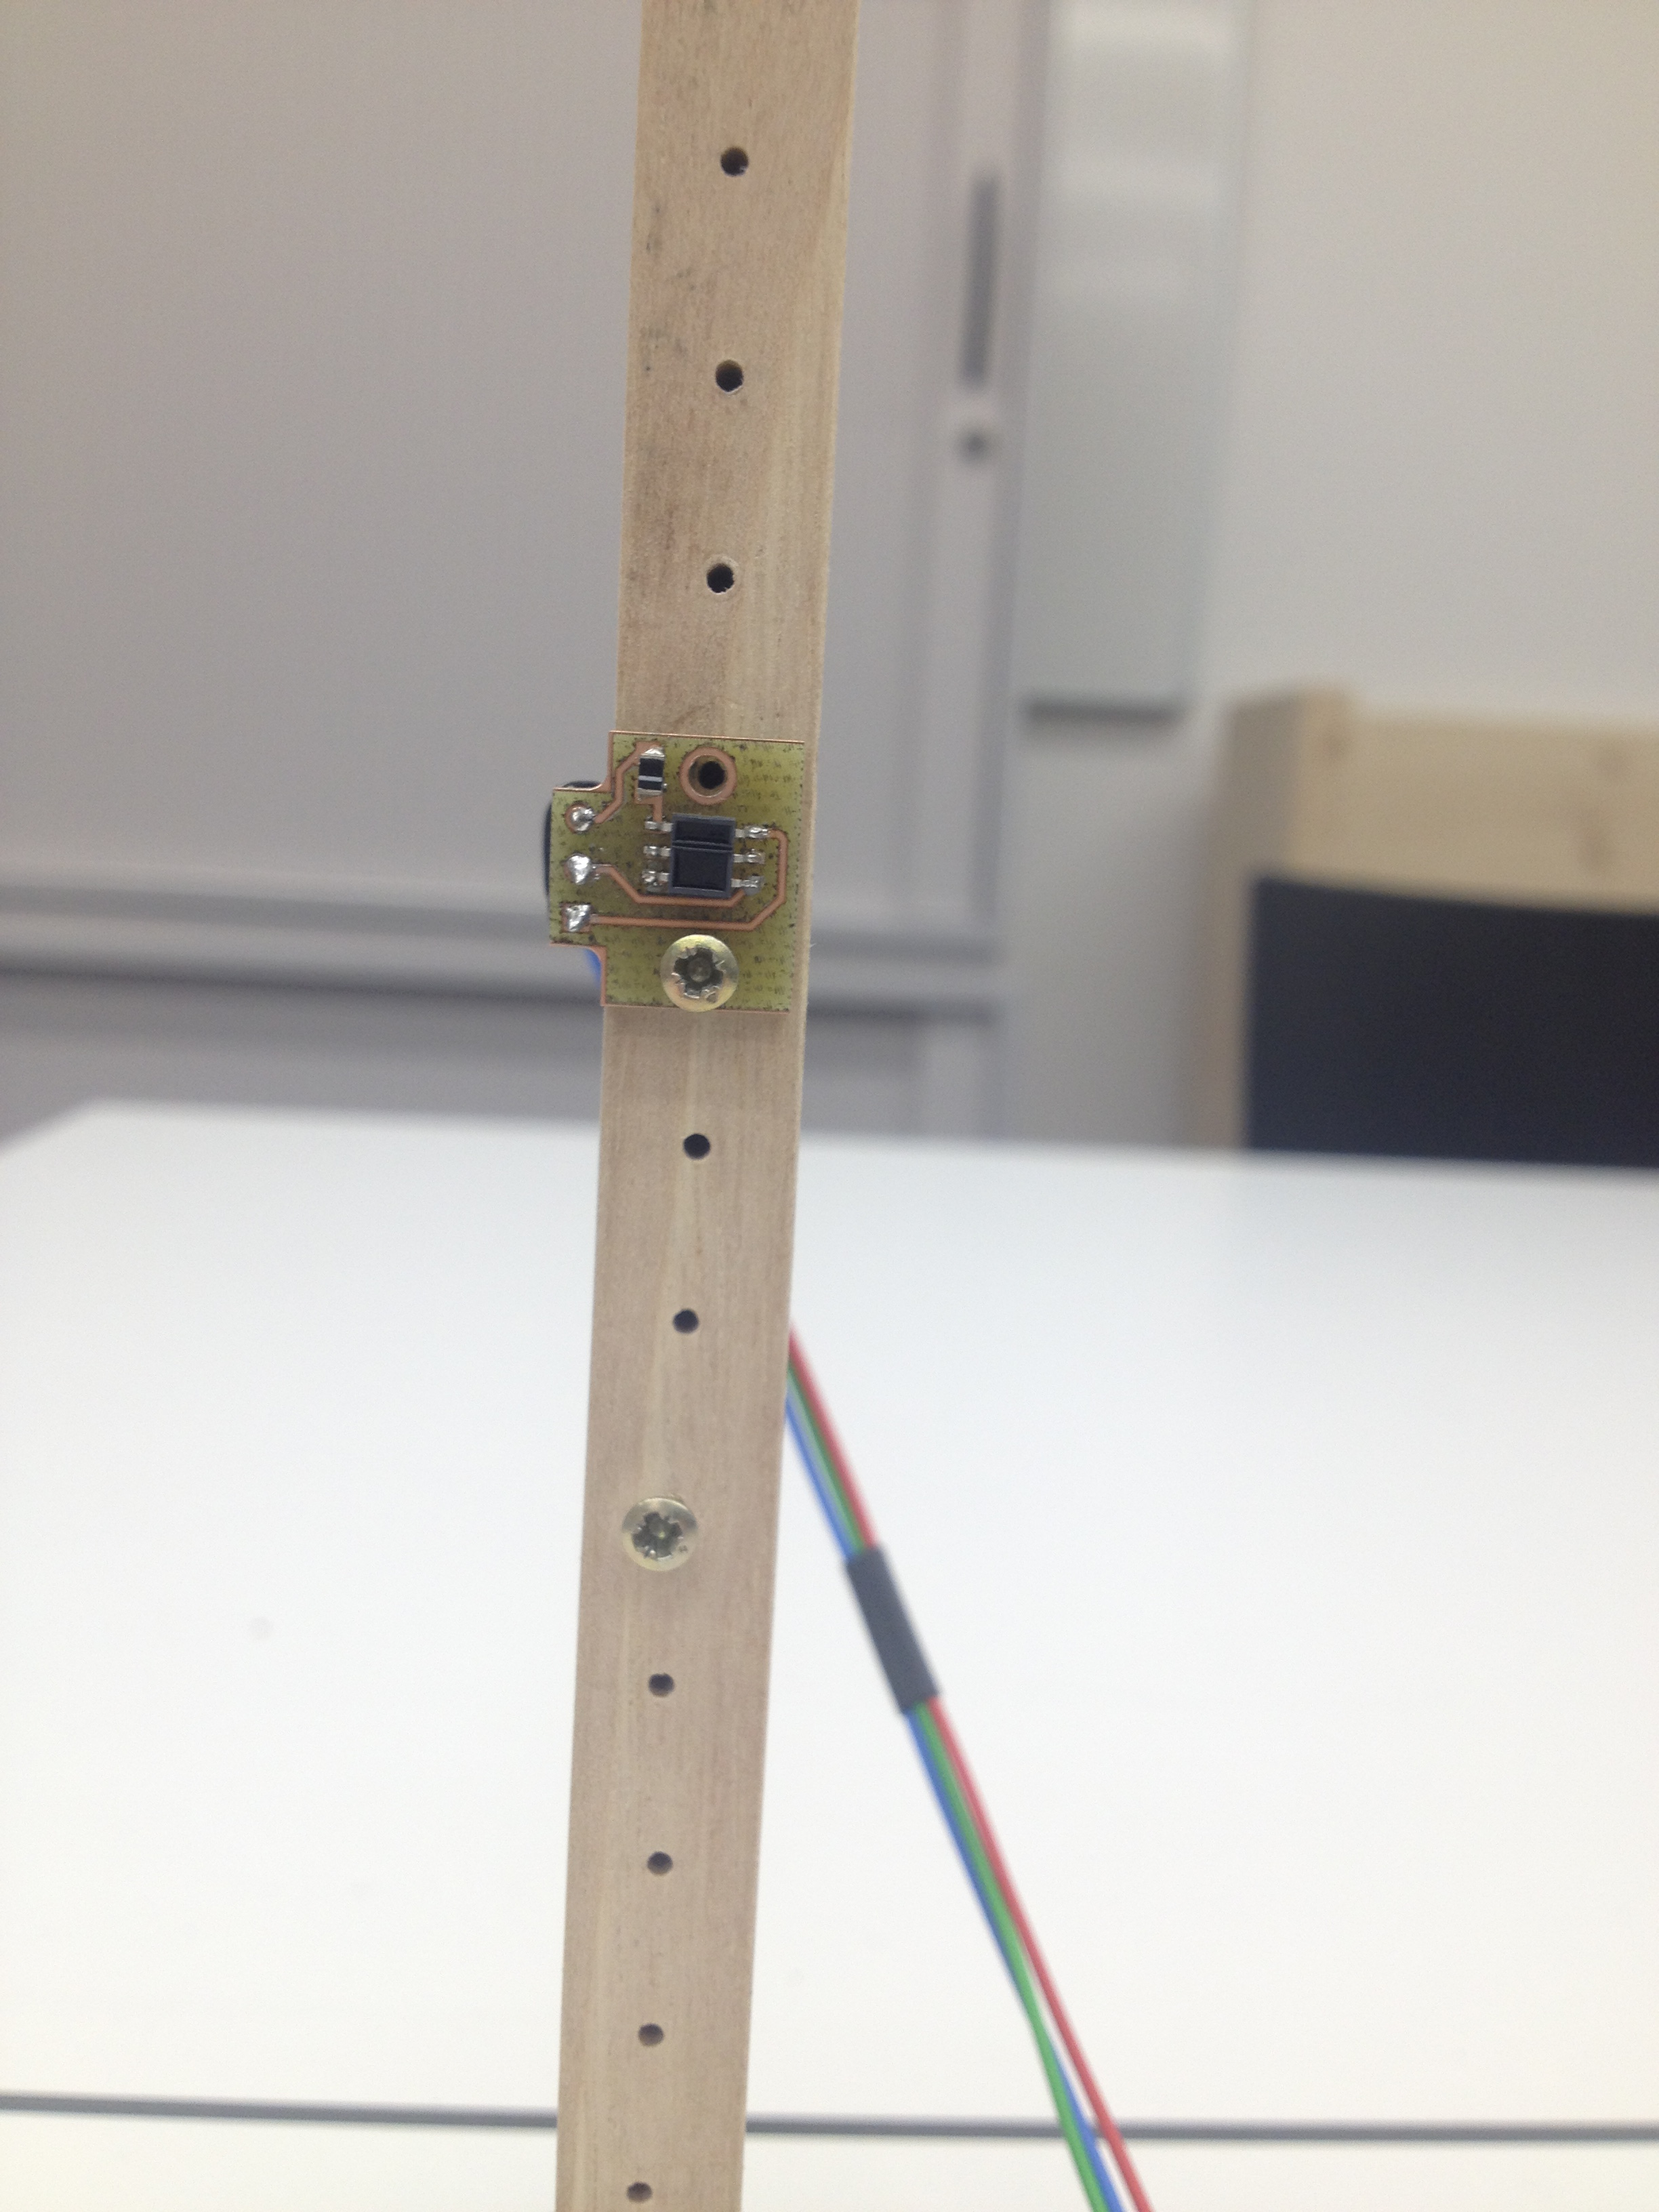
\includegraphics[width=.4\textwidth]{Sensor_Detail}
		\caption{Aufbau des Sensors für die Pendelmessung}
		\label{fig:Sensor_overview}
	\end{figure}